%%%%%%%%%%%%%%%%%%%%%%%%%%%%%%%%%%%%%%%%%%%%%%%%%%%%%%%%%%%%%%%%%%%%%%%%%%%%%%%%
%%                                                                
%%      SWSC LaTeX class for Journal of Space Weather and Space Climate
%%      
%%                                      (c) Springer-Verlag HD
%%                                      revised by EDP Sciences
%%                                      further revised by J. Watermann 
%%
%%%%%%%%%%%%%%%%%%%%%%%%%%%%%%%%%%%%%%%%%%%%%%%%%%%%%%%%%%%%%%%%%%%%%%%%%%%%%%%%
%%
%%      This demonstration file was derived from aa.dem
%%  
%%      AA vers. 7.0, LaTeX class for Astronomy & Astrophysics
%%      demonstration file
%%                                                (c) Springer-Verlag HD
%%                                                revised by EDP Sciences
%%
%%%%%%%%%%%%%%%%%%%%%%%%%%%%%%%%%%%%%%%%%%%%%%%%%%%%%%%%%%%%%%%%%%%%%%%%%%%%%%%%
%%
%%      modified for Journal of Space Weather and Space Climate
%%      by Jurgen Watermann, Editorial Advisor to SWSC
%%
%%      01-04-2012
%%      02-04-2012 revision 1
%%      12-07-2012 revision 2
%%      06-12-2012 revision 3 
%%      01-01-2014 revision 4
%%      06-03-2014 revision 4.1
%%
%%%%%%%%%%%%%%%%%%%%%%%%%%%%%%%%%%%%%%%%%%%%%%%%%%%%%%%%%%%%%%%%%%%%%%%%%%%%%%%%
%%
%%      The two sub-figures referenced in this template are of eps and png type,
%%      respectively, in order to demonstrate the usepackages subfigure and
%%      epstopdf and thus create pdf-only output 
%%
%%      If you want to use TexLive or MikTex together with a bibtex bibliography 
%%      file you may run Latex2e from the command line 
%%          pdflatex -shell-escape swsc.tex
%%          bibtex swsc (do not include an extension such as .tex or .bib)
%%          pdflatex -shell-escape swsc.tex
%%          pdflatex -shell-escape swsc.tex
%%
%%      A double call to pdflatex after calling bibtex is necessary in order to
%%      set citations and references correctly and insure that foreward/backward  
%%      linkage (backref option) is properly applied
%%      If you use MikTex you may need to make a triple call to pdflatex
%%
%%      If you are using TexLive or MikTex but not a bibtex type of bibliography
%%      you may simply run Latex2e twice from the command line 
%%          pdflatex -shell-escape swsc.tex
%%          pdflatex -shell-escape swsc.tex
%%
%%%%%%%%%%%%%%%%%%%%%%%%%%%%%%%%%%%%%%%%%%%%%%%%%%%%%%%%%%%%%%%%%%%%%%%%%%%%%%%%
%%
%%   single column 12-point version for review
%%

%%  with traditional abstract
\documentclass[referee,a4paper,12pt,traditabstract]{swsc} 

%%  with structured abstract 
%\documentclass[referee,a4paper,12pt,structabstract]{swsc} 

\usepackage{graphicx}
\usepackage{txfonts}
\usepackage{subfigure}
\usepackage{epstopdf}
\usepackage{lineno}
\usepackage[authoryear,round]{natbib}
\usepackage[backref]{hyperref}
\usepackage{url}
\usepackage[inline]{enumitem}
%%    This version assumes using bibtex with the swsc bibliography style file
\bibliographystyle{swsc.bst}

\hypersetup{colorlinks=true,citecolor=cyan,urlcolor=cyan,linkcolor=blue}

%%%%%%%%%%%%%%%%%%%%%%%%%%%%%%%%%%%%%%%%%%%%%%%%%%%%%%%%%%%%%%%%%%%%%%%%%%%%%%%%

\begin{document}

\begin{linenumbers}

   \title{Gaussian Processes Autoregressive Models for the Disturbance Storm Time Index}

   %\subtitle{I. Overviewing the $\kappa$-mechanism}
   
   \titlerunning{Gaussian Process $D_{st}$ models}

   \authorrunning{Chandorkar and Camporeale}

   \author{M. Chandorkar
          \inst{1}
          \and
          E. Camporeale\inst{1}
          }

   \institute{Centrum Wiskunde Informatica (CWI), Amsterdam,
              1098XG Amsterdam\\
              \email{\href{mailto:m.h.chandorkar@cwi.nl}{m.h.chandorkar@cwi.nl} \href{mailto:e.camporeale@cwi.nl}{e.camporeale@cwi.nl}} 
             }

%%   \date{Received September 15, 1996; accepted March 16, 1997}

  % \abstract{}{}{}{}{}        %% uncomment if structured abstract is desired
 %% 5 {} token are mandatory
 
   %% replace by pair of curly brackets, {}, if structured abstract is selected
   
   
   \abstract{
    We aim to improve the state of the art of \emph{One Step Ahead}(OSA) prediction of the $D_{st}$ geomagnetic activity index. In the domain of OSA prediction, it is well known that $D_{st}(t)$ values correlate strongly with values one hour in the past (i.e. $D_{st}(t-1)$). While a number of forecasting models have been proposed and compared, none of them have been compared with the \emph{Persistence} model to quantify their performance improvements above this most trivial of predictors. In this study we train Gaussian Process regression models for One Step Ahead (OSE) prediction of the Disturbance Storm Time ($D_{st}$) geomagnetic index. We propose three variants of the Gaussian Process model.
    \begin{enumerate*}
      \item Gaussian Process Auto regressive GP-AR 
      \item Gaussian Process Auto regressive with eXogenous inputs GP-ARX. 
    \end{enumerate*}
    We compare the performance of these models with the current state of the art in one step ahead $D_{st}$ prediction on a set of 
    63 benchmark storms from 1998-2006. The proposed Gaussian Process models not only outperform the rest but also the \emph{Persistence} model.
    }

   \keywords{Geomagnetic indices --
            $D_{st}$ OSA Prediction --
            Gaussian Processes --
            Machine Learning
            }

   \maketitle
%%
%%________________________________________________________________

\section{Introduction}



We use the hourly resolution Omni data set (see \cite{OmniPaper}) as extracted from NASA/GSFC's OMNI data set through OMNIWeb.
   
  
\section{Methodology: Gaussian Process}

We restrict ourselves to the supervised learning problem in statistics, which is inductive. In other words, we aim to model functions of single or multiple variables (i.e. fields $f(\mathbf{x}), \ x \in \mathbb{R}^d $), using a set of labeled data points ${(\mathbf{x}_i, y_i), \forall i \in 1 \cdots N}$. These problems have been studied extensively in statistics over the past century.

\emph{Stochastic Processes} extend the idea of probability distributions to the space of functions of a single or multiple variables. A \emph{Gaussian Process} is a stochastic process whose finite dimensional distributions are multivariate Gaussian \ref{eq:sto}.
\vspace{-\baselineskip}
\begin{eqnarray}
 \left(f(\mathbf{x}_1), f(\mathbf{x}_2) \cdots f(\mathbf{x}_N) \right)^T & \sim & \mathcal{N}\left(\mathbf{\mu}, \mathbf{\Lambda} \right) \label{eq:sto} \\
 \mathbf{\Lambda}_{ij} & = & K(\mathbf{x}_i, \mathbf{x}_j) \label{eq:kern}\\
 f & \sim & \mathcal{GP}(m(\mathbf{x}), K(\mathbf{x},\mathbf{x}'))
\end{eqnarray}

The covariance structure of a \emph{stochastic process} is represented by a symmetric positive definite function as given in \ref{eq:kern}. By \emph{Kolmogorov's extension theorem} (\citet{tao2011introduction}), the function $K: \mathbb{R}^d \times \mathbb{R}^d \rightarrow \mathbb{R}$ uniquely determines the process. Therefore this covariance function (also called kernel function in machine learning) helps us to specify the class of functions represented by the process.


\emph{Gaussian Processes} first appeared in machine learning research as the limiting case of Bayesian inference performed on neural networks with infinitely many neurons in the hidden layers \citet{Neal:1996:BLN:525544}. It was noted by the author that "there may be simpler ways to do inference in this case". Although their inception in the machine learning community is recent, they were studied in statistics/mathematics community as special cases of \emph{Stochastic Processes}. The reader is requested to refer to \cite{Rasmussen:2005:GPM:1162254} for an in depth treatment of Gaussian Processes in Machine Learning.  

\subsection{Formulation}

\begin{eqnarray}
      \mathbf{x} & \in & \mathbb{R}^d \\
      \mathbf{X} & = & (\mathbf{x}_1, \mathbf{x}_2, \cdots, \mathbf{x}_N) \\
      \mathbf{y} & = & (y_1, y_2, \cdots, y_N) \\
      y & = & f(\mathbf{x}) + \epsilon  \\
      f & \sim & \mathcal{GP}(m(\mathbf{x}), K(\mathbf{x},\mathbf{x}'))  \\
      \left(\mathbf{y} \ \ \mathbf{f_*} \right)^\intercal & \sim & 
\mathcal{N}\left(\mathbf{0}, \left[ \begin{array}{cc} \mathbf{K}(\mathbf{X}, \mathbf{X}) + \sigma^{2} \mathbf{I} & \mathbf{K}(\mathbf{X}, \mathbf{X_*}) \\ \mathbf{K}(\mathbf{X_*}, \mathbf{X}) & \mathbf{K}(\mathbf{X_*}, \mathbf{X_*}) \end{array} \right ] \right)
\end{eqnarray}


\subsection{Inference and Predictions}

\begin{eqnarray}
      \mathbf{f_*}|\mathbf{X},\mathbf{y},\mathbf{X_*} & \sim & \mathcal{N}(\mathbf{\bar{f}_*}, \Sigma_*)  \label{eq:posterior} \\
      \mathbf{\bar{f}_*} & = & \mathbb{E}[\mathbf{f_*}|\mathbf{X},\mathbf{y},\mathbf{X_*}]  \\
      & = & K(\mathbf{X_*},\mathbf{X})^\intercal [K(\mathbf{X},\mathbf{X}) + \sigma^{2} \mathbf{I}]^{-1} \mathbf{y} \\
      \Sigma_* & = & K(\mathbf{X_*}, \mathbf{X_*}) - K(\mathbf{X_*},\mathbf{X})^\intercal \left(K(\mathbf{X},\mathbf{X}) + \sigma^{2} \mathbf{I}\right)^{-1}K(\mathbf{X},\mathbf{X_*})
\end{eqnarray}


\subsection{Kernel Functions}

For the success of a Gaussian Process model an appropriate choice of kernel function is paramount. It is important to note that every kernel function generates a \emph{Reproducing Kernel Hilbert Space} (RKHS) of functions, and the nature of the kernel dictates what restrictions exist on the functions belonging to its RKHS. The Gaussian Process model essentially uses basis functions from this RKHS to represent the unknown function. The interested reader is suggested to refer to \cite{Berlinet2004} for a thorough treatment on RKHS and the rich theory behind them.

Some common kernel functions used in machine learning are.

\subsubsection{Radial Basis Function (RBF)}

The RBF kernel is the most commonly used kernel in machine learning, in its core it encodes the idea of \emph{smoothness} because functions drawn from its Hilbert space are infinitely differentiable. The RBF kernel is also an example of a \emph{stationary} kernel i.e. its value depends only on $||\mathbf{x} - \mathbf{y}||$. The quantity $\sigma$ is known as the characteristic \emph{length scale} of this kernel, it is a free parameter (also known as hyper-parameter) which must be determined by the modeller, refer to section \ref{sec:hyp} on how suitable values of kernel hyper-parameters.

\begin{equation}
    K(\mathbf{x}, \mathbf{y}) = \frac{1}{2} exp(-||\mathbf{x} - \mathbf{y}||^2/\sigma^2)
\end{equation}
    
    
\subsubsection{Polynomial}

The polynomial kernel is also a common kernel function employed in research, it has two hyper-parameters the degree $d$ and an intercept $b$. The polynomial kernel formulates the function approximation in terms of polynomial expansions of the input dimensions $\mathbf{x}$, more specifically it considers all monomial combination of the input dimensions up to degree $d$. When $d = 1$ it corresponds to a Bayesian linear regression model. 

\begin{equation}
    K(\mathbf{x}, \mathbf{y}) = (\mathbf{x}^\intercal \mathbf{y} + b)^d 
\end{equation}


In this study, we construct Gaussian Process models with polynomial kernels for \emph{one step ahead} prediction of the $D_{st}$ index. 


\subsection{Optimizing Hyper-parameters} \label{sec:hyp}

With kernel based prediction models one always encounters the crucial question of what values to assign to the kernel hyper-parameters. This is known as \emph{model tuning} in kernel research parlance. There are many methods to perform \emph{model tuning}, one generally formulates an objective function and aims to optimize it in terms of the hyper-parameters. Common examples of objective functions include data likelihood, cross validation performance scores and validation set performance scores among others. Since the objective function for the model tuning problem is non-convex and non-smooth in general, gradient free approaches are used to find approximate values of local optima.

The simplest way to perform model tuning is called \emph{grid search} which entails evaluating the above objective function on a fixed grid which is constructed by making a list of values for each hyper-parameter and taking the combinations of all such values. There are more sophisticated methods for \emph{model tuning} such as \emph{coupled simulated annealing} (\citet{Xavier-De-Souza2010}) and \emph{simplex search} (\citet{Nelder1965}) but they are computationally more expensive. In this study we chose \emph{grid search} as the model tuning routine. 

\section{One Step Ahead Prediction}



\subsection{Gaussian Process Nonlinear Auto-Regressive (GP-AR)}

The input vector $x_t$ at each time step is the $p$ order time history of $D_{st}$.
  \begin{eqnarray}
    D_{st}(t) & = & f(x_t) + \epsilon\\
    x_t & = & \left(D_{st}(t-1), D_{st}(t-2), \cdots , D_{st}(t-p)\right) \\
    f(x_t) & \sim & \mathcal{GP}(m(x_t), K(x_t,x_s)) \label{eq:DstGP}
\end{eqnarray}

\subsection{Gaussian Process Nonlinear Auto-Regressive with eXogenous inputs (GP-ARX)}

Solar wind velocity $V$ and interplanetary magnetic field $B_z$ recorded at the ACE satellite are used as the exogenous inputs of the model, along with the time history of $D_{st}$.
    
  \begin{eqnarray}
    & D_{st}(t) & = f(\mathbf{x}_t) + \epsilon \\
        & \mathbf{x}_t & = (D_{st}(t-1), D_{st}(t-2), \cdots , D_{st}(t-p), \\
        & \ \ \ \ \ & V(t-1), V(t-2), \cdots, V(t-p),\\
        & \ \ \ \ \ & B_{z}(t-1), B_{z}(t-2), \cdots, B_{z}(t-p))\\
    & f(x_t) & \sim \mathcal{GP}(m(\mathbf{x}_t), K(\mathbf{x}_t,\mathbf{x}_s)) \label{eq:DstGP1}
\end{eqnarray}



\section{Experiments}

   \begin{table}
      \caption[]{Opacity sources.}
         \label{KapSou}
     $$ 
         \begin{array}{p{0.5\linewidth}l}
            \hline
            \noalign{\smallskip}
            Source      &  T / {[\mathrm{K}]} \\
            \noalign{\smallskip}
            \hline
            \noalign{\smallskip}
            \citet{Ji2012} & \leq 1700^{\mathrm{a}}     \\
            \citet{kocijan2015modelling}                     & 1700 \leq T \leq 5000 \\
            \citet{Berlinet2004}                  & 5000 \leq             \\
            \noalign{\smallskip}
            \hline
         \end{array}
     $$ 
\begin{list}{}{}
\item[$^{\mathrm{a}}$] This is footnote a
\end{list}
\end{table}

\section{Results}
%%  This two-panel figure was inserted by JFW to demonstrate the subfigure and epstopdf packages


\begin{figure}
   \centering
   \subfigure{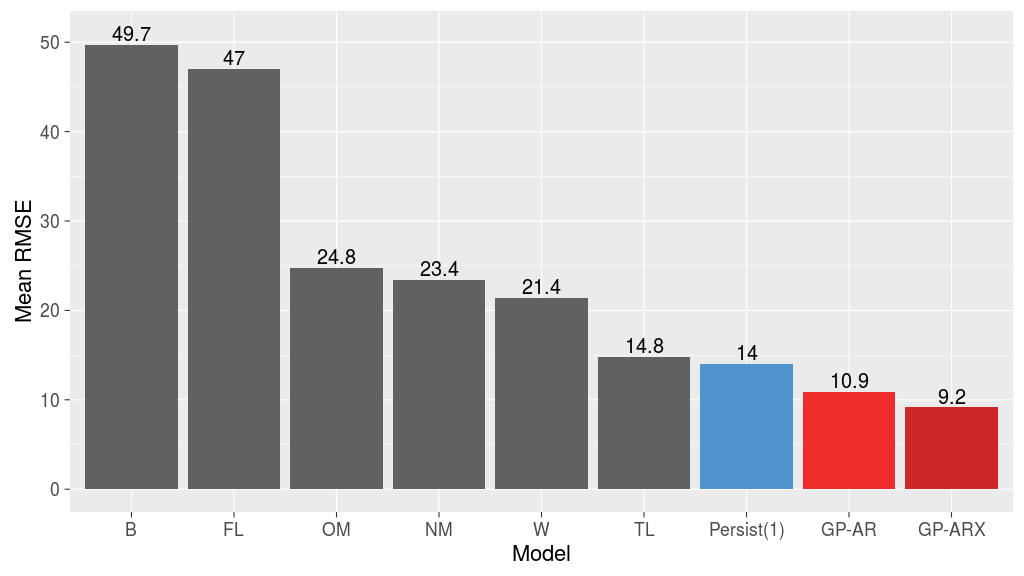
\includegraphics[width=\columnwidth]{Compare_RMSE.png}}
   \vspace{12pt}
   \subfigure{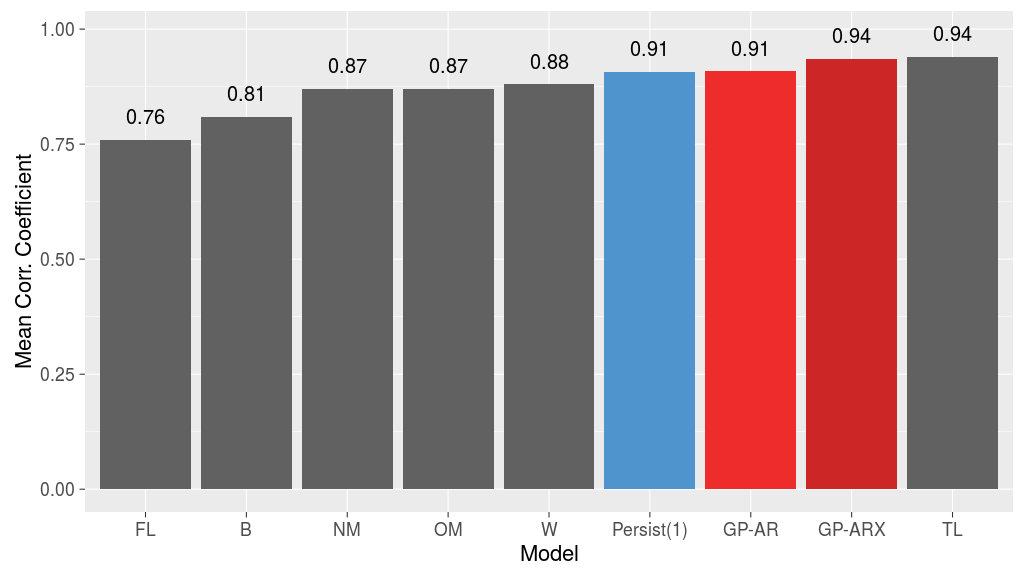
\includegraphics[width=\columnwidth]{Compare_CC.png}}
   \caption{\small  Performance Comparison} 
   \label{fig:rmsecc}
   \end{figure}

\begin{figure}
   \centering
   \subfigure{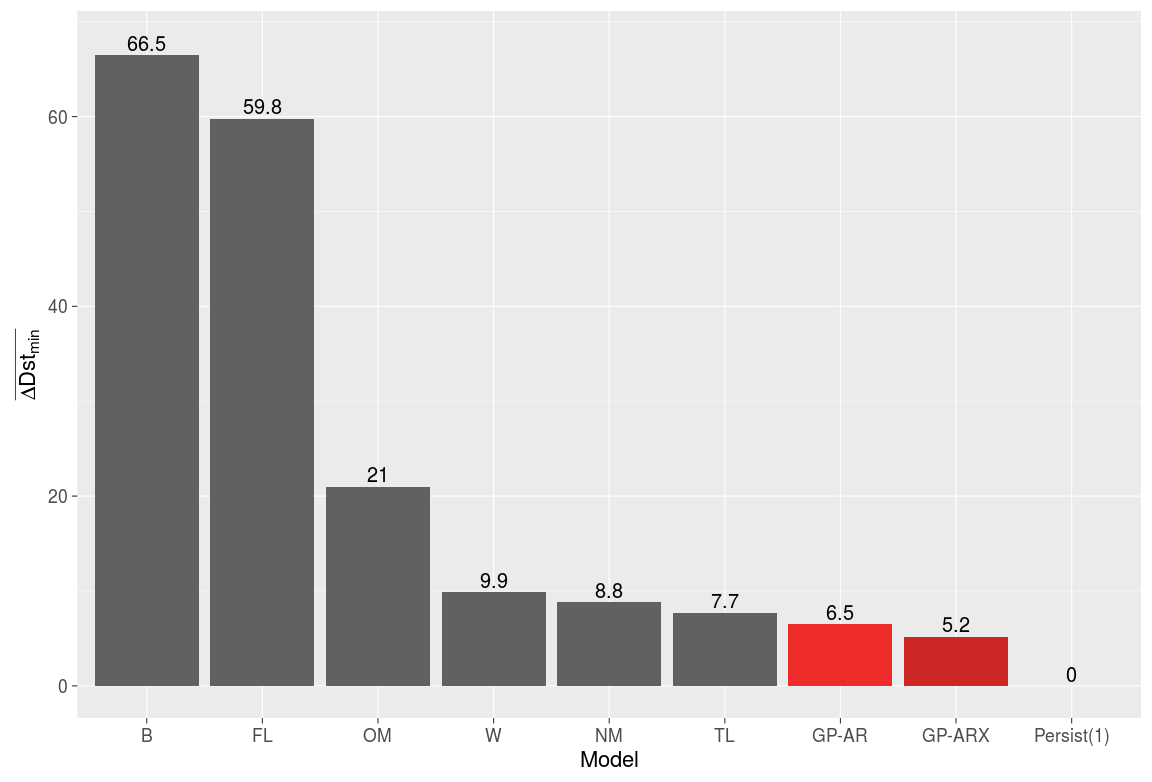
\includegraphics[width=\columnwidth]{Compare_deltaDst.png}}
   \vspace{12pt}
   \subfigure{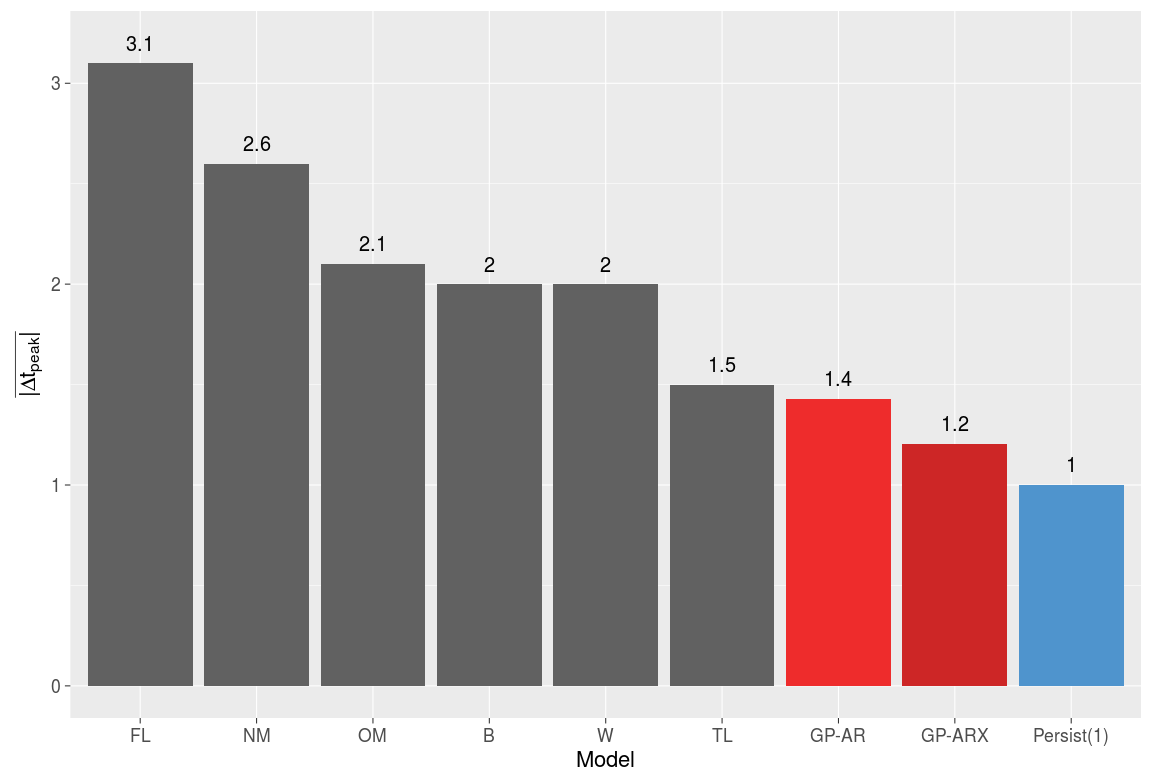
\includegraphics[width=\columnwidth]{Compare_timingerr.png}}
   \caption{\small  Performance Comparison} 
   \label{fig:deltaDst}
   \end{figure}

\section{Conclusions}

   \begin{enumerate}
      \item Persistence model due to \emph{One Step Ahead} restriction 
      \item Superior performance of \emph{Gaussian Process} NAR and NARX models
      \item Multi step ahead prediction should be the preferred gold standard with respect to forecasting of geomagnetic indices.
   \end{enumerate}

\begin{acknowledgements}
      We acknowledge use of NASA/GSFC's Space Physics Data Facility's OMNIWeb (or CDAWeb or ftp) service, and OMNI data.
\end{acknowledgements}

%%    This version assumes use of bibtex with the swsc.bib file being present
%%    If your bib file has a different name you need to change the following line

\bibliography{swsc}

\end{linenumbers}

\end{document}

%%    If you wish to include your bibliography items in your tex file 
%%    using {thebibliography} as shown below you must out-comment the 
%%    three lines above (insert % at the start of each line) 

\begin{thebibliography}{}

   \bibitem[Baker(1966)]{baker} Baker, N., Solar Evolution,
      in Stellar Evolution, ed.\ R. F. Stein and A. G. W. Cameron,
      Plenum, New York, 333, 1966.

   \bibitem[Balluch(1988)]{balluch} Balluch, M., A paper on something, 
      {\it Astron. Astrophys}, {\bf 200}, 58-63, 1988.

   \bibitem[Cox(1980)]{cox} Cox, J. P.,
      Theory of Stellar Pulsation,
      Princeton University Press, Princeton, 1980.

   \bibitem[Cox and Stewart(1969)]{cox69} Cox, A. N., and J. N. Stewart,
      Academia Nauk, {\it Scientific Information}, {\bf 15}, 1-11, 1969.

   \bibitem[Dumm and Kopf(2014)]{dummkopf} Dumm, Z., and Z. Kopf, A new self-inconsistent 
      core stability model, 
      {\it J. Space Weather Space Clim.}, {\bf 4}, A00, 2014, DOI: 10.1051/swsc/2014000,
      \url{http://dx.doi.org/10.1051/swsc/2014000}.

   \bibitem[Fool(2012)]{fool} Fool, X. Y., All earlier results are wrong, 
      {\it J. Space Weather Space Clim.}, {\bf 2}, A00, 2012, DOI: 10.1051/swsc/2012000,
      \url{http://dx.doi.org/10.1051/swsc/2012000}.

   \bibitem[Fou(2013)]{fou} Fou, Y. X., No earlier results were right, 
      {\it J. Space Weather Space Clim.}, {\bf 3}, A00, 2013, DOI: 10.1051/swsc/2013000,
      \url{http://dx.doi.org/10.1051/swsc/2013000}.

   \bibitem[Kr\"ugel et al.(1971)]{krugel71} Kr\"ugel, A. H., A. F. Davidsen, D. Tytler, and G. A. Kriss, 
      Summary of Project Achievements, Technical Report 08-11, 
      Fake Company, Nowherecity, Nowhereland, 1971.

   \bibitem[Mizuno(1980)]{mizuno} Mizuno, H., A further step backward in scientific understanding, 
      {\it Prog. Theor. Phys.}, {\bf 64}, 544-545, 1980.
   
   \bibitem[Tscharnuter(1987)]{tscharnuter} Tscharnuter, W. M., Who knows about astronomy?, 
      {\it Astron. Astrophys}, {\bf 188}, 55-57, 1987.

   \bibitem[Yorke(1980a)]{yorke80a} Yorke, H. W., A paper on nothing, 
      {\it Astron. Astrophys}, {\bf 86}, 286, 1980a.

   \bibitem[Yorke(1980b)]{yorke80b} Yorke, H. W., A paper on everything, 
      {\it Astron. Astrophys}, {\bf 86}, 291, 1980b.

\end{thebibliography}

\end{linenumbers}

\end{document}

%%%%%%%%%%%%%%%%%%%%%%%%%%%%%%%%%%%%%%%%%%%%%%%%%%%%%%%%%%%%%%%%%%%%%%%%%%%
%%
%%   Below are examples of how to use particular document layout features
%%
%%%%%%%%%%%%%%%%%%%%%%%%%%%%%%%%%%%%%%%%%%%%%%%%%%%%%%%%%%%%%%%%%%%%%%%%%%%
%%  Examples for figures using graphicx
%%  A guide "Using Imported Graphics in LaTeX2e"  (Keith Reckdahl)
%%  is available on a lot of LaTeX public servers or ctan mirrors.
%%  The file is : epslatex.pdf 
%%%%%%%%%%%%%%%%%%%%%%%%%%%%%%%%%%%%%%%%%%%%%%%%%%%%%%%%%%%%%%%%%%%%%%%%%%%

%_____________________________________________________________
%                 A figure as large as the width of the column
%-------------------------------------------------------------
   \begin{figure}
   \centering
   \includegraphics[width=\textwidth]{empty.eps}
      \caption{Vibrational stability equation of state
               $S_{\mathrm{vib}}(\lg e, \lg \rho)$.
               $>0$ means vibrational stability.
              }
         \label{FigVibStab}
   \end{figure}
%
%_____________________________________________________________
%                                    One column rotated figure
%-------------------------------------------------------------
   \begin{figure}
   \centering
   \includegraphics[angle=-90,width=3cm]{empty.eps}
      \caption{Vibrational stability equation of state
               $S_{\mathrm{vib}}(\lg e, \lg \rho)$.
               $>0$ means vibrational stability.
              }
         \label{FigVibStab}
   \end{figure}
%
%_____________________________________________________________
%                        Figure with caption on the right side 
%-------------------------------------------------------------
   \begin{figure}
   \centering
   \includegraphics[width=3cm]{empty.eps}
      \caption{Vibrational stability equation of state
               $S_{\mathrm{vib}}(\lg e, \lg \rho)$.
               $>0$ means vibrational stability.
              }
         \label{FigVibStab}
   \end{figure}
%
%_____________________________________________________________
%
%_____________________________________________________________
%                                Figure with a new BoundingBox 
%-------------------------------------------------------------
   \begin{figure}
   \centering
   \includegraphics[bb=10 20 100 300,width=3cm,clip]{empty.eps}
      \caption{Vibrational stability equation of state
               $S_{\mathrm{vib}}(\lg e, \lg \rho)$.
               $>0$ means vibrational stability.
              }
         \label{FigVibStab}
   \end{figure}
%
%_____________________________________________________________
%
%_____________________________________________________________
%                                      The "resizebox" command 
%-------------------------------------------------------------
   \begin{figure}
   \resizebox{\textwidth}{!}
            {\includegraphics[bb=10 20 100 300,clip]{empty.eps}
      \caption{Vibrational stability equation of state
               $S_{\mathrm{vib}}(\lg e, \lg \rho)$.
               $>0$ means vibrational stability.
              }
         \label{FigVibStab}
   \end{figure}
%
%______________________________________________________________
%
%_____________________________________________________________
%                                             Simple A&A Table
%_____________________________________________________________
%
\begin{table}
\caption{Nonlinear Model Results}             % title of Table
\label{table:1}      % is used to refer this table in the text
\centering                          % used for centering table
\begin{tabular}{c c c c}        % centered columns (4 columns)
\hline\hline                 % inserts double horizontal lines
HJD & $E$ & Method\#2 & Method\#3 \\    % table heading 
\hline                        % inserts single horizontal line
   1 & 50 & $-837$ & 970 \\      % inserting body of the table
   2 & 47 & 877    & 230 \\
   3 & 31 & 25     & 415 \\
   4 & 35 & 144    & 2356 \\
   5 & 45 & 300    & 556 \\ 
\hline                                   %inserts single line
\end{tabular}
\end{table}
%
%_____________________________________________________________
%                                             Two column Table 
%_____________________________________________________________
%
\begin{table*}
\caption{Nonlinear Model Results}             
\label{table:1}      
\centering          
\begin{tabular}{c c c c l l l }     % 7 columns 
\hline\hline       
                      % To combine 4 columns into a single one 
HJD & $E$ & Method\#2 & \multicolumn{4}{c}{Method\#3}\\ 
\hline                    
   1 & 50 & $-837$ & 970 & 65 & 67 & 78\\  
   2 & 47 & 877    & 230 & 567& 55 & 78\\
   3 & 31 & 25     & 415 & 567& 55 & 78\\
   4 & 35 & 144    & 2356& 567& 55 & 78 \\
   5 & 45 & 300    & 556 & 567& 55 & 78\\
\hline                  
\end{tabular}
\end{table*}
%
%-------------------------------------------------------------
%                                          Table with notes 
%-------------------------------------------------------------
%
% A single note
\begin{table}[h]
\caption{\label{t7}Spectral types and photometry for stars in the
  region.}
\centering
\begin{tabular}{lccc}
\hline\hline
Star&Spectral type&RA(J2000)&Dec(J2000)\\
\hline
69           &B1\,V     &09 15 54.046 & $-$50 00 26.67\\
49           &B0.7\,V   &*09 15 54.570& $-$50 00 03.90\\
LS~1267~(86) &O8\,V     &09 15 52.787&11.07\\
24.6         &7.58      &1.37 &0.20\\
\hline
LS~1262      &B0\,V     &09 15 05.17&11.17\\
MO 2-119     &B0.5\,V   &09 15 33.7 &11.74\\
LS~1269      &O8.5\,V   &09 15 56.60&10.85\\
\hline
\end{tabular}
\tablefoot{ The top panel shows likely members of Pismis~11. The second
panel contains likely members of Alicante~5. The bottom panel
displays stars outside the clusters.}
\end{table}
%
% More notes
%
\begin{table}[h]
\caption{\label{t7}Spectral types and photometry for stars in the
  region.}
\centering
\begin{tabular}{lccc}
\hline\hline
Star&Spectral type&RA(J2000)&Dec(J2000)\\
\hline
69           &B1\,V     &09 15 54.046 & $-$50 00 26.67\\
49           &B0.7\,V   &*09 15 54.570& $-$50 00 03.90\\
LS~1267~(86) &O8\,V     &09 15 52.787&11.07\tablefootmark{a}\\
24.6         &7.58\tablefootmark{1}&1.37\tablefootmark{a}   &0.20\tablefootmark{a}\\
\hline
LS~1262      &B0\,V     &09 15 05.17&11.17\tablefootmark{b}\\
MO 2-119     &B0.5\,V   &09 15 33.7 &11.74\tablefootmark{c}\\
LS~1269      &O8.5\,V   &09 15 56.60&10.85\tablefootmark{d}\\
\hline
\end{tabular}
\tablefoot{ The top panel shows likely members of Pismis~11. The second
panel contains likely members of Alicante~5. The bottom panel
displays stars outside the clusters.\\
\tablefoottext{a}{Photometry for MF13, LS~1267 and HD~80077 from
Dupont et al.}
\tablefoottext{b}{Photometry for LS~1262, LS~1269 from
Durand et al.}
\tablefoottext{c}{Photometry for MO2-119 from
Mathieu et al.}
}
\end{table}
%
%-------------------------------------------------------------
%                                       Table with references 
%-------------------------------------------------------------
%
\begin{table*}[h]
 \caption[]{\label{nearbylistaa2}List of nearby SNe used in this work.}
\begin{tabular}{lccc}
 \hline \hline
  SN name &
  Epoch &
 Bands &
  References \\
 &
  (with respect to $B$ maximum) &
 &
 \\ \hline
1981B   & 0 & {\it UBV} & 1\\
1986G   &  $-$3, $-$1, 0, 1, 2 & {\it BV}  & 2\\
1989B   & $-$5, $-$1, 0, 3, 5 & {\it UBVRI}  & 3, 4\\
1990N   & 2, 7 & {\it UBVRI}  & 5\\
1991M   & 3 & {\it VRI}  & 6\\
\hline
\noalign{\smallskip}
\multicolumn{4}{c}{ SNe 91bg-like} \\
\noalign{\smallskip}
\hline
1991bg   & 1, 2 & {\it BVRI}  & 7\\
1999by   & $-$5, $-$4, $-$3, 3, 4, 5 & {\it UBVRI}  & 8\\
\hline
\noalign{\smallskip}
\multicolumn{4}{c}{ SNe 91T-like} \\
\noalign{\smallskip}
\hline
1991T   & $-$3, 0 & {\it UBVRI}  &  9, 10\\
2000cx  & $-$3, $-$2, 0, 1, 5 & {\it UBVRI}  & 11\\ %
\hline
\end{tabular}
\tablebib{(1)~\citet{branch83};
(2) \citet{phillips87}; (3) \citet{barbon90}; (4) \citet{wells94};
(5) \citet{mazzali93}; (6) \citet{gomez98}; (7) \citet{kirshner93};
(8) \citet{patat96}; (9) \citet{salvo01}; (10) \citet{branch03};
(11) \citet{jha99}.
}
\end{table}
%_____________________________________________________________
%                                 A rotated Table in landscape  
%  In the preamble, use:   \usepackage{lscape}
%-------------------------------------------------------------
\begin{landscape}
\begin{table*}
\caption{Summary for ISOCAM sources with mid-IR excess 
(YSO candidates).}\label{YSOtable}
\centering
\begin{tabular}{crrlcl} 
\hline\hline             
ISO-L1551 & $F_{6.7}$~[mJy] & $\alpha_{6.7-14.3}$ 
& YSO type$^{d}$ & Status & Comments\\
\hline
  \multicolumn{6}{c}{\it New YSO candidates}\\ % To combine 6 columns into a single one
\hline
  1 & 1.56 $\pm$ 0.47 & --    & Class II$^{c}$ & New & Mid\\
  2 & 0.79:           & 0.97: & Class II ?     & New & \\
  3 & 4.95 $\pm$ 0.68 & 3.18  & Class II / III & New & \\
  5 & 1.44 $\pm$ 0.33 & 1.88  & Class II       & New & \\
\hline
  \multicolumn{6}{c}{\it Previously known YSOs} \\
\hline
  61 & 0.89 $\pm$ 0.58 & 1.77 & Class I & \object{HH 30} & Circumstellar disk\\
  96 & 38.34 $\pm$ 0.71 & 37.5& Class II& MHO 5          & Spectral type\\
\hline
\end{tabular}
\end{table*}
\end{landscape}
%
%_____________________________________________________________
%                              Table longer than a single page  
%  In the preamble, use:              \usepackage{longtable}
%-------------------------------------------------------------
%          All long tables have to be placed at the end, after 
%                                        \end{thebibliography}
%
% In the text, at the place where the large table should appear
% add the command:
\addtocounter{table}{1}
% Tables counters will be well numbered.
%
\end{thebibliography}
% If table 2
\longtab{2}{
\begin{longtable}{lllrrr}
\caption{\label{kstars} Sample stars with absolute magnitude}\\
\hline\hline
Catalogue& $M_{V}$ & Spectral & Distance & Mode & Count Rate \\
\hline
\endfirsthead
\caption{continued.}\\
\hline\hline
Catalogue& $M_{V}$ & Spectral & Distance & Mode & Count Rate \\
\hline
\endhead
\hline
\endfoot
%%
Gl 33    & 6.37 & K2 V & 7.46 & S & 0.043170\\
Gl 66AB  & 6.26 & K2 V & 8.15 & S & 0.260478\\
Gl 68    & 5.87 & K1 V & 7.47 & P & 0.026610\\
         &      &      &      & H & 0.008686\\
Gl 86 
\footnote{Source not included in the HRI catalog. See Sect.~5.4.2 for details.}
         & 5.92 & K0 V & 10.91& S & 0.058230\\
\end{longtable}
}% End \longtab
%
%_____________________________________________________________
%                              Table longer than a single page
%                                             and in landscape 
%  In the preamble, use:       \usepackage{longtable,lscape}
%-------------------------------------------------------------
%          All long tables have to be placed at the end, after
%                                        \end{thebibliography}
%
% In the text, at the place where the large table should appear
% add the command:                        
\addtocounter{table}{1} 
% Tables counters will be well numbered.
%
\end{thebibliography}
% If table 2
\longtabL{2}{
\begin{landscape}
\begin{longtable}{lllrrr}
\caption{\label{kstars} Sample stars with absolute magnitude}\\
\hline\hline
Catalogue& $M_{V}$ & Spectral & Distance & Mode & Count Rate \\
\hline
\endfirsthead
\caption{continued.}\\
\hline\hline
Catalogue& $M_{V}$ & Spectral & Distance & Mode & Count Rate \\
\hline
\endhead
\hline
\endfoot
%%
Gl 33    & 6.37 & K2 V & 7.46 & S & 0.043170\\
Gl 66AB  & 6.26 & K2 V & 8.15 & S & 0.260478\\
Gl 68    & 5.87 & K1 V & 7.47 & P & 0.026610\\
         &      &      &      & H & 0.008686\\
Gl 86
\footnote{Source not included in the HRI catalog. See Sect.~5.4.2 for details.}
         & 5.92 & K0 V & 10.91& S & 0.058230\\
\end{longtable}
\end{landscape}
}% End \longtabL
%
% Online Material
%_____________________________________________________________
%        Online appendices have to be placed at the end, after
%                                        \end{thebibliography}
%-------------------------------------------------------------
\end{thebibliography}

\Online

\begin{appendix} %First online appendix
\section{Background galaxy number counts and shear noise-levels}
Because the optical images used in this analysis...

\begin{figure*}
\centering
\includegraphics[width=16.4cm,clip]{1787f24.ps}
\caption{Plotted above...}
\label{appfig}
\end{figure*}

Because the optical images...
\end{appendix}

\begin{appendix} %Second online appendix
These studies, however, have faced...
\end{appendix}

\end{document}
%
%_____________________________________________________________
%        Some tables or figures are in the printed version and
%                      some are only in the electronic version
%-------------------------------------------------------------
%
% Leave all the tables or figures in the text, at their right place 
% and use the commands \onlfig{}{} and \onltab{}{}. These elements
% will be automatically placed at the end, in the section
% Online material.

\documentclass{swsc}
...
\begin{document}
text of the paper...
\begin{figure*}%f1
\includegraphics[width=10.9cm]{1787f01.eps}
\caption{Shown in greyscale is a...}
\label{cl12301}}
\end{figure*}
...
from the intrinsic ellipticity distribution.
% Figure 2 available electronically only
\onlfig{2}{
\begin{figure*}%f2
\includegraphics[width=11.6cm]{1787f02.eps}
\caption {Shown in greyscale...}
\label{cl1018}
\end{figure*}
}

% Figure 3 available electronically only
\onlfig{3}{
\begin{figure*}%f3
\includegraphics[width=11.2cm]{1787f03.eps}
\caption{Shown in panels...}
\label{cl1059}
\end{figure*}
}

\begin{figure*}%f4
\includegraphics[width=10.9cm]{1787f04.eps}
\caption{Shown in greyscale is...}
\label{cl1232}}
\end{figure*}

\begin{table}%t1
\caption{Complexes characterisation.}\label{starbursts}
\centering
\begin{tabular}{lccc}
\hline \hline
Complex & $F_{60}$ & 8.6 &  No. of  \\
...
\hline
\end{tabular}
\end{table}
The second method produces...

% Figure 5 available electronically only
\onlfig{5}{
\begin{figure*}%f5
\includegraphics[width=11.2cm]{1787f05.eps}
\caption{Shown in panels...}
\label{cl1238}}
\end{figure*}
}

As can be seen, in general the deeper...
% Table 2 available electronically only
\onltab{2}{
\begin{table*}%t2
\caption{List of the LMC stellar complexes...}\label{Properties}
\centering
\begin{tabular}{lccccccccc}
\hline  \hline
Stellar & RA & Dec & ...
...
\hline
\end{tabular}
\end{table*}
}

% Table 3 available electronically only
\onltab{3}{
\begin{table*}%t3
\caption{List of the derived...}\label{IrasFluxes}
\centering
\begin{tabular}{lcccccccccc}
\hline \hline
Stellar & $f12$ & $L12$ &...
...
\hline
\end{tabular}
\end{table*}
}
%
%-------------------------------------------------------------
%     For the online material, table longer than a single page
%                 In the preamble, use: \usepackage{longtable}
%       or for landscape option: \usepackage{longtable,lscape}
%-------------------------------------------------------------
\documentclass{swsc}
\usepackage[varg]{txfonts}
\usepackage{graphicx}
\usepackage{longtable}

\begin{document}
text of the paper
% Table will be print automatically at the end, in the section Online material.
\onllongtab{3}{
\begin{longtable}{lrcrrrrrrrrl}
\caption{Line data and abundances ...}\\
\hline
\hline
Def & mol & Ion & $\lambda$ & $\chi$ & $\log gf$ & N & e &  rad & $\delta$ & $\delta$ 
red & References \\
\hline
\endfirsthead
\caption{Continued.} \\
\hline
Def & mol & Ion & $\lambda$ & $\chi$ & $\log gf$ & B & C &  rad & $\delta$ & $\delta$ 
red & References \\
\hline
\endhead
\hline
\endfoot
\hline
\endlastfoot
A & CH & 1 &3638 & 0.002 & $-$2.551 &  &  &  & $-$150 & 150 &  Jorgensen et al. (1996) \\                    
\end{longtable}
}% End onllongtab

% Or for landscape, large table:

\onllongtabL{3}{
\begin{landscape}
\begin{longtable}{lrcrrrrrrrrl}
...
\end{longtable}
\end{landscape}
}% End onllongtabL

